\section{Architecture and source of the Internet}

Starting of this study is done with a small introduction. Since the thesis and the research question~\ref{ssec:research_question} focus on the networking aspect and more specifically on Internet we must first declare what exactly this is how it has come to be. In this section we will handle the origin and evolution of the Internet, other alternatives to Internet and some of the issues with the current Internet. 

\subsection{Origin and evolution of the current Internet}

\begin{figure}[H]
    \centering
    \includegraphics[width=0.7\textwidth]{figures/Internettimeline}
    \caption{Timeline of the Internet \citep{website:Internethistory}} 
    \label{fig:Internettimeline}
\end{figure}
\npar

Internet started out as research aimed at packet switch in the early 1960s. The name of the very first packet switching network was called ARPANET (Advanced Research Projects Agency NETwork), this was a data network established in the USA. While research began early 1960s, it was first established in 1969. The main difference between circuit switching and packet switching is that in packet switching one line of communication can be used for many different packets. These packets can have different sources and/or different destinations, this formed the base of packet switching networks. The first ever packet switched network was set up in California on 29 October 1969 \citep{petersalus1995}. It was commonly thought that ARPANET was set up to survive a nuclear blast, but in fact it was set up as a proof-of-concept and could handle a partial network failure \citep{katiehafner1998}. Later it became clear that this type of network was very robust and was praised for it's ability to withstand partial network failures \citep{janetabbate2000}.
\npar
\begin{figure}[H]
    \centering
    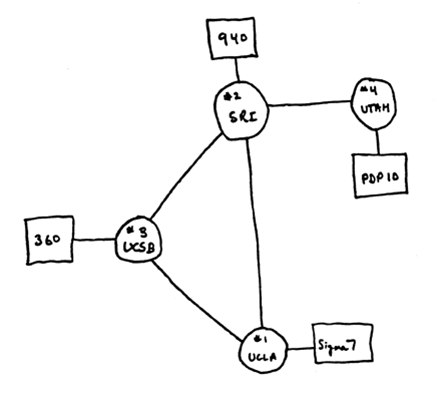
\includegraphics{figures/earlyarpanet}
    \caption{Early version of ARPANET \citep{pwp:rinaintro}} 
    \label{fig:earlyarpanet}
\end{figure}
\npar
After the first proof of concept ARPANET quickly expanded during the 1970s. It both expanded on the protocol it used and on the amount of connected nodes. We must first notice that in ARPANET there was no talk of client/server, it was originally designed as a peer-to-peer network \citep{petersalus2008, timbernerslee2000}. ARPANET also went outside the boundaries of the USA when it connected to a Norwegian node in 1973. Later other nodes were included such as a node in Britain, Sweden, \ldots (see image~\ref{fig:latearpanet}. The packet switching network left the proof-of-concept phase in 1975 when it was declared operational \citep{petersalus2008}. While the technology that ARPANET was run on is currently unimportant, the significance of the protocol that was used in this early network deemed to be humongous.  
\npar
When ARPANET was first launched in 1969 it used the 1822 protocol \citep{frankheart1970}, it was named after the report number. This protocol was designed to work cross-architecture and consisted of several fields: a message type, host address (numerical), and a data field. Messages were sent across the network using early routers, called: \emph{Interface Message Processors}. These devices were the early versions of routers. The entire system worked with either a direct, local link where messages were unicasted or were further broadcasted to other IMPs. Once the message had been successfully delivered and acknowledgment was sent back across the network to the sender. ARPANET was entirely designed for this protocol but on top of this protocol the NCP (Network Control Program) protocol was added which in essence meant that more layers added. These protocols were deemed outdated in 1983 when the transition was made to TCP/IP a huge amount of changes were required\footnote{Hence why this is one of the most notable \emph{flag days} in history of software}.
\npar
\begin{figure}[H]
    \centering
    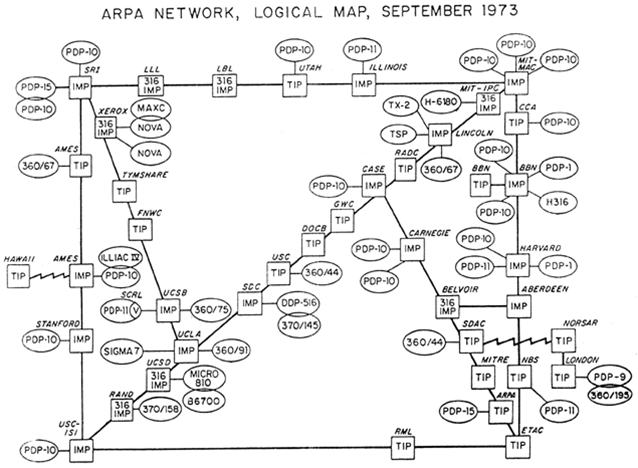
\includegraphics[width=0.8\textwidth]{figures/latearpanet}
    \caption{Late version of ARPANET \citep{vrijders2014prototyping}} 
    \label{fig:latearpanet}
\end{figure}
\npar
In 1983 the transition was made towards the currently used TCP/IP protocol. This marked the start of the early \emph{Internet}. TCP/IP stands for Transport Control Protocol / Internet Protocol. This means it is in fact two protocols, transport layer protocol (TCP) and Internet Layer protocol (IP). ARPANET also allowed for layering of higher-level protocols and this is where the OSI model was born. ARPANET decommissioned in 1990 when the transition towards the current Internet had been made. This was mainly due the rise of ISPs (Internet Service Providers) in the late 1980s and 1990s. We can see that ARPANET was essential in the birth of the current Internet. 
\npar
In later years the Internet became a standardized product. Several standardization bodies regulate the current Internet. The one responsible for the TCP/IP standards is the Internet Engineering Task Force (IETF\footnote{\url{http://www.ietf.org/}}). While ISO (International Organization for Standards) is responsible for the overarching 7-layer model. Since the bottom part of the 5-layer model and the 7-layer model is exactly the same and we will be working close to the bottom, we will not be discussing the differences between these models further.


\subsection{Previous alternatives}

One of the most notable alternatives to ARPANET was the French-developed CYCLADES. It was created shortly after the birth of ARPANET. The main reason of this research project was to explore alternatives to ARPANET. The core principle was still the same though as also this network was a packet switching network. Some concepts from CYCLADES were later applied to the current version of the Internet, such as: host-responsibility and end-to-end protocol. 
\npar
At the time in the 1970s several research networks were developed. While all these networks were packet switching, the main point of argument was the role of network or host. Either the network or the host had to be responsible to deliver the packet and this divided the early networks in two groups. Other early research networks on packet switching were: DECnet, EIN nee COST II, EPSS, GEIS, IPX/SPX, Merit Network, \ldots. These networks were very similar to ARPANET and did not feature any noticeable new changes. The most important of these alternatives was CYCLADES and most of the flaws that ARPANET showed were filled by using technology and research from CYCLADES.

\subsection{Shortcomings of the current Internet}
\label{ssec:Internet_shortcomings}

The current model of Internet shows quite a few shortcomings. The main reason here is that the original protocols were never revised or alternatives were never considered. This static approach has lead to the use of a lot of hacks, patches, band-aids, \ldots. A very recent and obvious example is the need currently required to change from IPv4 towards IPv6. The reason for this is that we are simply running out of IPv4 addresses and thus we need another protocol to handle this. The question then rises: why do we need so many changes to a system that should be scalable? This questions can easily be answered when we look at the history of the Internet. It is based on a rigid system with very little science behind it. When we take a close look at the OSI model\ref{fig:OSImodel} we see a huge number of protocols who all have to work in conjunction with each other and overlap in several occasions\footnote{Example: IPv4 and IPv6 overlap}. 

\begin{figure}[H]
    \centering
    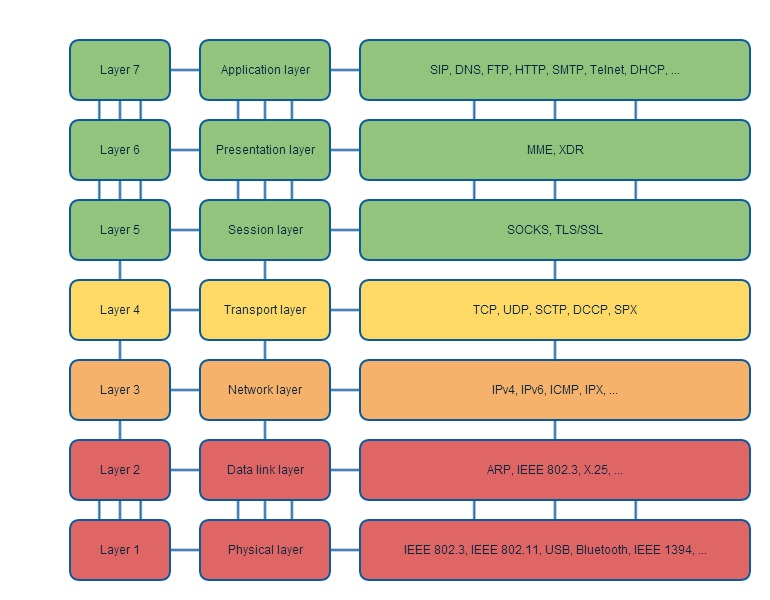
\includegraphics[width=\textwidth]{figures/osilayer}
    \caption{OSI model with examples} 
    \label{fig:OSImodel}
\end{figure}

\npar

Some examples of these issues in the current Internet are: multihoming, denial-of-service, port mapping, NAT (Network Address Translation), IP geomapping, \ldots. While some of these issues are solvable, they require a number of band-aids on the current Internet. This stems from the origin of the Internet. While it started out as a research net it was almost instantly made to be a production network. This was done while other networks, such as CYCLADES, were still researching and solving obvious problems. Due to faulty decisions the Internet continued to be build on these protocols and thus became flawed from the start. For example it is currently impossible to send a packet to two unique destinations (IP addresses), this requires you to send two different packets. This also causes problems with mobility where targets change IP addresses quickly when running through different Internet providing cells. Handovers from routers is a big hassle for mobile users and slows down the entire process of staying online permanently. While short interruptions are not an issue when loading a website, it can prove fatal when using this Internet for live communications, monitoring, \ldots. Proper multihoming can potentially fix this issue, but this is currently very hard to achieve in the current state of the Internet. 
\npar
Another example is the use of NAT, Network Address Translation. This is needed because we are currently running out of IPv4 addresses and it enables small networks to have multiple nodes connected to the Internet at the same time. The problem is that this only solves issues in one direction. People from outside of the network can no longer see the people behind the NAT-router. This causes issues for several applications, such as peer-to-peer applications and many others. It also means that the router is actually breaching the model because it alters packets (specific port number and ip). In the normal model this is never changed between end hosts.
\npar
\begin{figure}[H]
    \centering
    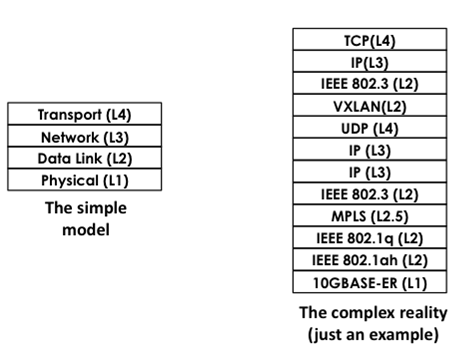
\includegraphics[width=0.9\textwidth]{figures/layeractualexamplenorina}
    \caption{Example of the current Internet layer system \citep{pwp:rinaintro}} 
    \label{fig:layeractualexamplenorina}
\end{figure}
\npar
Further issues become apparent when looking at common items in some layers. We see that it is possible to map IP-addresses to geological information, thus violating privacy of the people using the Internet. Secondly when an attacker obtains an IP-address it becomes quite easy for this attacker to spam this IP with data causing a disruption in the service of the host. This is known as: Denial-of-Service Attack. Other mapping problems are the common application-port mapping that occurs. When anybody intercepts a packet he can read the port number and deduce for what application that packet can be used. This leads to more privacy issues and limits applications in their use as they are not free to choose a port number. 
\npar
We see that the current Internet has quite a lot of issues and can use a general, uniform model or architecture as an answer. Continuing down the road of constantly applying band-aids to a already broken system is clearly not an answer. A clear slate is need and this is where the research question will try to find an answer to. 

